


\documentclass[a4paper,11pt]{article}

\usepackage{amsmath,amssymb} %symbole matematyczne
\usepackage[T1]{fontenc} %język: znaki, literki
\usepackage[utf8]{inputenc} %język: system kodowania tekstu
\usepackage[polish]{babel}
\usepackage{hyperref}
\usepackage{booktabs}
\usepackage{amsmath}
\usepackage{amsfonts}
\usepackage{amssymb}
\usepackage[comma]{natbib}
\usepackage{graphicx} % (pozwala uzyc pdf jpg png)
\title{Informatyka geodezyjna - projekt 1}
\author{ Hubert Mizura\\
	312155 gr 3a}

\begin{document}
	\title{INFORMATYKA GEODEZYJNA \\ 
		
		PROJEKT 1 \\
		
		(transformacje)}
	
	\author{ Hubert Mizura\\
		312155 gr 3a}
	\maketitle
	\newpage
	\section{Działanie programu}
	\subsection{Funkcje oraz działanie}
	Program został stworzony w środowiksu spyder. Zawarte są dwa pliki, gdzie w jednym znajdują się funkcje niebędne do transformacji współrzędnych,a w drugim przedstawione jest działanie programu .
	\subsection{Import danych i transformacja}
	Dane są importowane z pliku tekstowego (notatnika), w kolejnym kroku tworzymy tablicę gdzie umiesczane są współrzędne. Na samym końcu program tworzy tablicy gdzie zostaną umieszczone wartości po transformacji.
	\begin{figure}
		\centering
		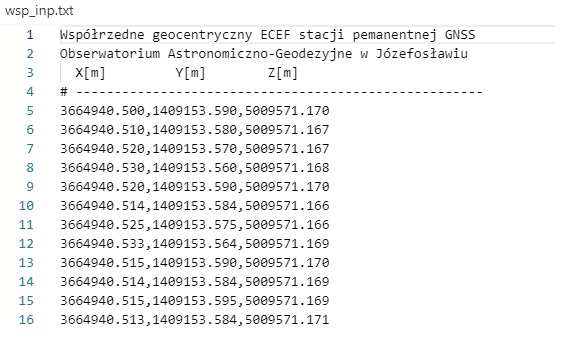
\includegraphics[width=10cm, height=5cm]{C:/Users/User/Documents/infa 2/proj 1 hubi/wsp.png}
		\caption{Współrzędne geocentryczne stacji GNSS w Józefosławiu}\label{fig:1}
	\end{figure}
	\subsection{Rodzaje funkcji}
	Możliwe jest dokonywanie kilku rodzajów przekształceń np. do współrzędnych geodezyjnych za pomocą algorytmu Hirvonena jak i również do układu 2000 i 1992.
	\newpage

	
	
	\tableofcontents	%spis tresci
		\paragraph{Repozytorium:}
	https://github.com/HubertMizura/Projekt-1-informatyka.git
\end{document}